\documentclass[11pt,letterpaper]{article}

\usepackage[utf8]{inputenc}
\usepackage[T1]{fontenc}
\usepackage{mathptmx} % Times font for academic look
\usepackage[margin=1in]{geometry}
\usepackage{amsmath,amssymb,amsfonts,bm}
\usepackage{booktabs}
\usepackage{graphicx}
\usepackage{float}
\usepackage[colorlinks=true,citecolor=blue,linkcolor=blue,urlcolor=blue]{hyperref}
\usepackage{xcolor}
\usepackage[font=small,labelfont=bf]{caption}
\setlength{\textfloatsep}{10pt plus 2pt minus 2pt}
\setlength{\floatsep}{8pt plus 2pt minus 2pt}
\setlength{\intextsep}{10pt plus 2pt minus 2pt}
\usepackage{subcaption}
\usepackage{tikz}
\usepackage{enumitem}
\usepackage{multicol}

\usetikzlibrary{calc, positioning, shapes.geometric, arrows.meta, fit, backgrounds}

% Standardize Colors
\definecolor{boxgray}{RGB}{240, 240, 240}
\definecolor{boxblue}{RGB}{220, 235, 250}
\definecolor{boxorange}{RGB}{255, 240, 220}
\definecolor{boxgreen}{RGB}{220, 250, 220}
\definecolor{cInFill}{HTML}{F2F2F2} \definecolor{cInLine}{HTML}{888888}
\definecolor{cAuFill}{HTML}{E3EDF7} \definecolor{cAuLine}{HTML}{3B6FA0}
\definecolor{cAdFill}{HTML}{FBEEDC} \definecolor{cAdLine}{HTML}{C07C33}
\definecolor{cEvFill}{HTML}{E4F1E8} \definecolor{cEvLine}{HTML}{3F8457}

% Custom commands
\newcommand{\bpb}{\text{BPB}}
\newcommand{\loss}{\mathcal{L}}
\newcommand{\nats}{\text{nats}}

\title{\LARGE \textbf{Back to Entropy: Evaluating Base Language Models\\ Beyond Perplexity and Benchmarks}}
\author{David Afonso Valente\\\normalsize Bottlecap AI}

\date{}

\begin{document}

\maketitle
\begin{abstract}
Base models are usually chosen from a scorecard of public benchmarks, which is an unreliable guide
for two reasons: the benchmarks are public before the model exists and unstable across evaluation
setups, and they score a model before adaptation, whereas teams deploy it after. Among candidates
within $2\times$ of each other in size, GSM8K picks the better model for a target domain $35.9\%$ of
the time and MMLU-Pro $40.0\%$, below chance by point estimate. We instead adapt every candidate to
recent text from the target domain under one small, identical budget and rank them by predictive loss
in bits per byte, a tokenizer-agnostic measurement that costs minutes per model. Against a criterion
built from each corpus's held-out text, this ranks candidates at least as well as every public
benchmark, of which only HellaSwag clears chance, across 17 models and a replication on four corpora;
its lead over ranking by parameter count is statistically resolved ($+0.250$, $[+0.074, +0.500]$,
lenient). The result carries to real systems: after fifteen models are fine-tuned on a news task,
adapted bits per byte ranks the resulting systems correctly in $0.949$ of size-matched pairs and
places every model within one rank of its final position. Code and artifacts are released.
\end{abstract}

\section{Introduction}
\label{sec:intro}
A new base model ships most weeks, and everyone who might use one---a research group, a company,
the team maintaining a product---asks the same question: \emph{how good is this model, for what we
do?} That is a measurement problem. What arrives with the model instead is a scorecard---MMLU-Pro,
HellaSwag, GSM8K---and reading it is the obvious thing to do.

Exams are the wrong class of instrument for it, for a structural reason rather than a matter of
benchmark quality. They were written by other people, for other purposes, and were public before the
model existed. A high score is therefore consistent with two very different situations: the model is
genuinely stronger, or the model saw more of that exam's subject matter during pre-training. No
reader can tell which, because pre-training mixtures are not disclosed. The consequence is visible
inside our own cohort: Llama-3.2-1B and Qwen2.5-1.5B are $2.1$ points apart on HellaSwag and
$3.4\%$ apart in adapted bits per byte, yet $55.3$ points apart on GSM8K. Two models can model
fresh English almost identically well and differ by almost a factor of ten on GSM8K. The scores are not even
stable: identical released weights move $-0.60$ to $+0.69$ GSM8K points when only the \emph{host}
changes, A100 to H100, and one decoding setting a checkpoint ships with was worth $9.86$ GSM8K points to
Gemma-4-12B in our own re-score (Appendix~\ref{app:rescore}).

And none of those exams is about your text. Measured against a criterion built
from a target domain's own documents, GSM8K and MMLU-Pro select the better of two similarly-sized
candidates $35.9\%$ and $40.0\%$ of the time by point estimate. A practitioner who reads them is not
getting weak evidence about their decision; they are getting evidence about a different decision.

The second problem is timing. Every exam scores a model exactly as it ships, but no team deploys a
model exactly as it ships: they adapt it to their data first. What matters is how good a model
\emph{becomes}, and a model that looks weak out of the box---one that has simply never seen prose
like yours---may need only a little adaptation to overtake one that looked stronger.

\paragraph{What we propose.} We propose measuring the model instead: predictive loss on text the
evaluator owns, after one small identical adaptation. Three properties make that work where per-token perplexity did not: \emph{bytes} rather than
tokens as the denominator, so vocabularies do not distort the comparison; \emph{fresh} text dated
after every candidate shipped, so the guarantee comes from the calendar rather than from trust; and
\emph{equal preparation}, one identical adaptation budget applied to every candidate before
measuring, which turns ``which model already writes like my corpus'' into ``which model gets there
fastest.'' Train-before-test \cite{zhang2025trainbeforetest} prepares candidates identically with
labelled benchmark data; we do it unsupervised, on fresh text, and in bytes.

\begin{center}
\fbox{\begin{minipage}{0.95\columnwidth}
\textbf{The minimum viable run.} Text from the target domain, dated after every candidate shipped,
is split $80/10/10$; the smallest corpus we report on is $15$\,MB. Every finalist is adapted with one
shared configuration---LoRA rank 16, $\alpha{=}32$, dropout $0.05$,
learning rate $10^{-4}$, effective batch 32, \texttt{all-linear} targets, 250 steps over
$512$-token blocks, which is $4.1$M training tokens seen per candidate---and candidates are ranked by
bits per byte on the held-out test split. On one A100 this cost $3.7$ GPU-minutes at $0.5$B, $11.6$ at
$7.7$B, $24.7$ at $12$B and $62.7$ at $31$B. We recommend treating a gap under $2\%$ as a tie, roughly
the measurement's own noise floor (Section~\ref{sec:using}). The GPU time is the cheap part;
assembling the corpus is the main cost, and text a product already generates needs only a clean split,
not a release date.
\end{minipage}}
\end{center}

Figure~\ref{fig:selectors} is the result, and it carries through to real systems: when fifteen
models are fine-tuned, adapted BPB, measured beforehand, places every one within a single rank of
where it finishes. Section~\ref{sec:protocol} gives the protocol and how we know the right ranking, Section~\ref{sec:results} the measurement, and
Section~\ref{sec:using} what to do with it. Every number in this paper recomputes from a committed
artifact:
\url{https://github.com/DavidAfonsoValente/entropy-bench}.
\begin{figure*}[t]
\centering
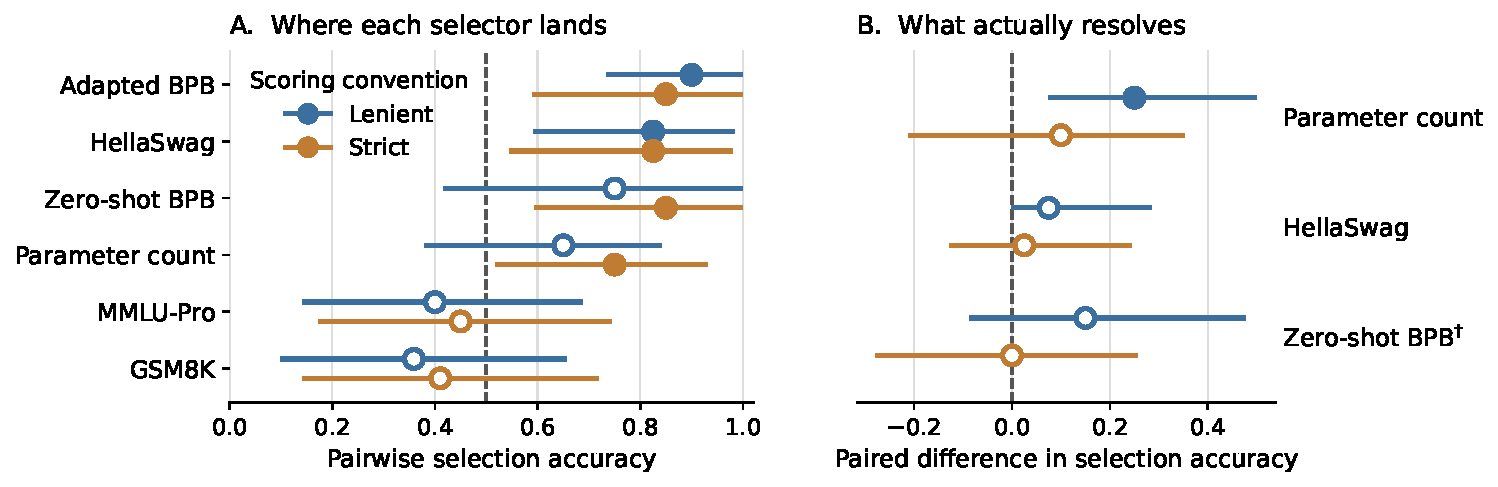
\includegraphics[width=\textwidth]{figures/fig_selectors.pdf}
\caption{\textbf{How often each way of choosing a base model picks the better one.} \emph{Extended
cohort: 17 models, $40$ size-matched pairs, news criterion.} Over the $40$ pairs of models within
$2\times$ in size, judged by an in-domain criterion built from the target
corpus's own held-out text (Section~\ref{sec:criterion}). \textbf{A} gives each selector's
accuracy: adapted BPB is top under lenient scoring and level with the unadapted reading under
strict, and both generative benchmarks fall below chance by point estimate. \textbf{B} gives the comparison the paper actually claims---the \emph{paired}
difference between adapted BPB and each baseline, on the same pairs. Intervals are $95\%$
cluster-bootstrap over models; a \textbf{hollow marker} means the interval still contains chance
(A) or zero (B), so that comparison has not resolved. At seventeen bootstrap units exactly one
has: adapted BPB over parameter count, $+0.250$ $[+0.074, +0.500]$ lenient.
Panel B plots \emph{adapted BPB minus the named baseline}, so
positive favours adaptation; the best public benchmark is HellaSwag.
$\dagger$~computed after the fact rather than preregistered.}
\label{fig:selectors}
\end{figure*}
\begin{figure*}[t]
\centering
\resizebox{0.97\textwidth}{!}{
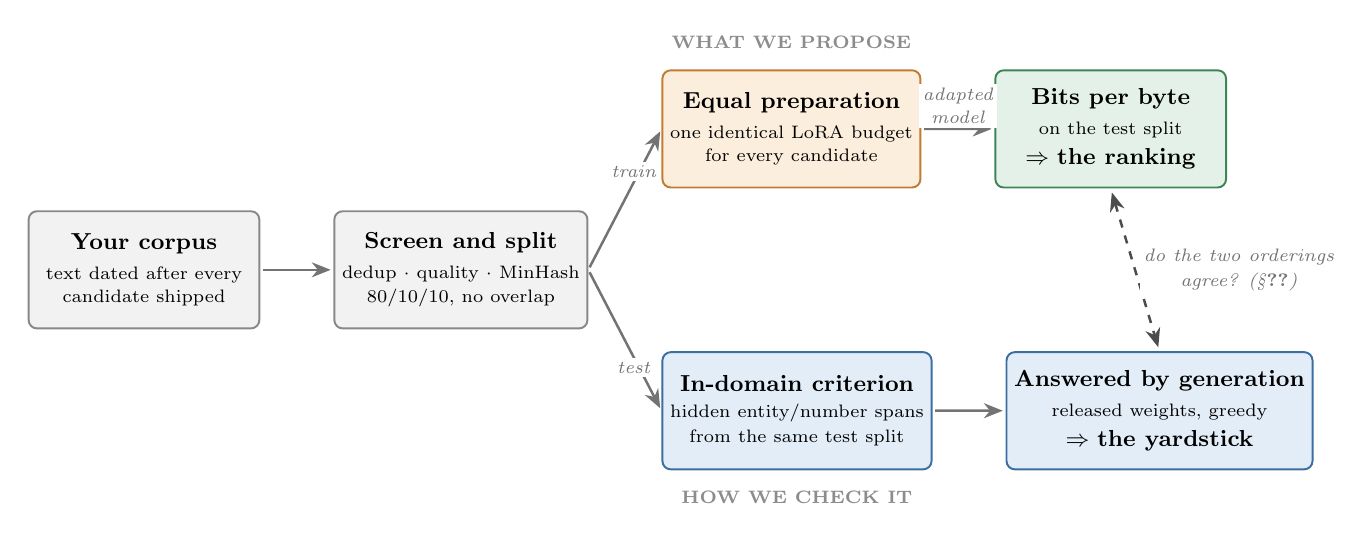
\begin{tikzpicture}[scale=0.93, transform shape,
  font=\small,
  >={Stealth[length=2.4mm,width=1.9mm]},
  stage/.style={draw, line width=0.7pt, rounded corners=3pt,
                minimum width=3.15cm, minimum height=1.6cm, align=center, inner sep=3pt},
  arm/.style={font=\scriptsize\bfseries, text=black!45},
  elbl/.style={font=\scriptsize\itshape, text=black!55, fill=white, inner sep=1.5pt},
  flow/.style={->, line width=0.9pt, draw=black!55, shorten >=1pt, shorten <=1pt}
]
\node[stage, fill=cInFill, draw=cInLine] (corpus)
  {\shortstack{\textbf{Your corpus}\\[2pt]{\scriptsize text dated after every}\\{\scriptsize candidate shipped}}};
\node[stage, fill=cInFill, draw=cInLine, right=1.0cm of corpus] (split)
  {\shortstack{\textbf{Screen and split}\\[2pt]{\scriptsize dedup $\cdot$ quality $\cdot$ MinHash}\\{\scriptsize 80/10/10, no overlap}}};

\node[stage, fill=cAdFill, draw=cAdLine, above right=0.30cm and 1.0cm of split] (adapt)
  {\shortstack{\textbf{Equal preparation}\\[2pt]{\scriptsize one identical LoRA budget}\\{\scriptsize for every candidate}}};
\node[stage, fill=cEvFill, draw=cEvLine, right=1.0cm of adapt] (bpb)
  {\shortstack{\textbf{Bits per byte}\\[2pt]{\scriptsize on the test split}\\[1pt]$\Rightarrow$ \textbf{the ranking}}};

\node[stage, fill=cAuFill, draw=cAuLine, below right=0.30cm and 1.0cm of split] (cloze)
  {\shortstack{\textbf{In-domain criterion}\\[2pt]{\scriptsize hidden entity/number spans}\\{\scriptsize from the same test split}}};
\node[stage, fill=cAuFill, draw=cAuLine, right=1.0cm of cloze] (gen)
  {\shortstack{\textbf{Answered by generation}\\[2pt]{\scriptsize released weights, greedy}\\[1pt]$\Rightarrow$ \textbf{the yardstick}}};

\node[arm, above=1.6mm of adapt] {WHAT WE PROPOSE};
\node[arm, below=1.6mm of cloze] {HOW WE CHECK IT};

\draw[flow] (corpus) -- (split);
\draw[flow] (split.east) -- node[elbl, above, pos=0.62]{train} (adapt.west);
\draw[flow] (split.east) -- node[elbl, below, pos=0.62]{test} (cloze.west);
\draw[flow] (adapt) -- node[elbl, above]{\shortstack{adapted\\model}} (bpb);
\draw[flow] (cloze) -- (gen);
\draw[<->, line width=0.9pt, draw=black!70, dashed, shorten >=1.5pt, shorten <=1.5pt] (bpb.south) -- node[elbl, right=0.5mm]{\shortstack{do the two orderings\\agree? (\S\ref{sec:mechanism})}} (gen.north);
\end{tikzpicture}
}
\caption{\textbf{The whole study on one page.} The upper arm is the protocol we propose: take text
from your own domain that postdates every candidate, screen and split it, adapt every candidate
under one identical budget, and rank by bits per byte on the held-out test split. The lower arm is
how we check that ranking without appealing to the benchmarks under criticism: the \emph{same}
held-out text supplies a criterion whose items are answered by generation from the released base
weights, so it is neither trainable-for nor scored by the quantity it validates. The paper is the
comparison of the two orderings.}
\label{fig:pipeline}
\end{figure*}
\section{The Protocol}
\label{sec:protocol}
Two things have to be built before any model can be ranked: the measurement, and the yardstick
that says whether a ranking is any good. Figure~\ref{fig:pipeline} shows both, and neither is
elaborate.

\subsection{Measuring: three phases}
\label{sec:phases}
The procedure is deliberately small enough to run on every candidate a team is considering. It has
three phases, in this order, and the ordering is load-bearing: the corpus is fixed and screened
before any model touches it.

\paragraph{Phase 1: the corpus.} Collect recent text from the target domain, dated after every
candidate's release. Deduplicate exactly, filter with Gopher quality heuristics, remove MinHash/LSH
near-duplicates at Jaccard $0.60$, and split 80/10/10 with no identifier or normalised-text overlap
across splits. For our primary snapshot---Google News, 8 June 2026, $119{,}054$ articles---we also
run three reference-free membership screens and quarantine the \emph{union} of everything any model
flags, so every candidate is measured on an identical retained corpus
(Appendix~\ref{app:criterion}). The other three corpora (Table~\ref{tab:corpora}) lean on the
calendar instead of a detector: Reddit and Hacker News are scraped in August 2026, after every model
in the cohort shipped, and the arXiv set runs from 9 June to 20 August, so its later documents do the
same work while its earliest sit alongside the news snapshot in time.

\paragraph{Phase 2: equal preparation.} Pack the retained training text into contiguous
$512$-token blocks and adapt every candidate with the \emph{same} configuration: LoRA
\cite{hu2021lora} rank 16, $\alpha{=}32$, dropout $0.05$, learning rate $10^{-4}$, effective batch
32, \texttt{all-linear} targets, 250 update steps. One shared configuration rather than a per-model
search is deliberate: a search we tried first handed small models more trials than large ones, a size
bias no correction removes (Appendix~\ref{app:robust}). One configuration suits no architecture
perfectly, but we prefer a bias we can name.

\paragraph{Phase 3: measure in bits per byte.} Compute cross-entropy on the held-out test split and
divide by the UTF-8 byte length $|B|$ of the text those predictions cover:
\begin{equation}
\bpb = \frac{\loss_{\text{nats}}}{\ln 2} \times \frac{|\text{Tokens}|}{|B|}
\label{eq:bpb}
\end{equation}
The denominator is the point: a model with a larger vocabulary spends fewer tokens on the same text
and looks better under per-token perplexity for free, where bytes are a physical property of the text
and identical for every candidate. Test blocks are independent and non-overlapping, so context resets
at every cut, and injected document-start markers stay available as context but are always masked as
prediction targets. Report both endpoints, before adaptation and after, because they answer different
questions (Section~\ref{sec:mechanism}).

\paragraph{Cohort and setup.} We evaluate 11 base checkpoints spanning dense Transformers, one
sparse MoE and one Liquid architecture (0.5B--35B parameters; Table~\ref{tab:leaderboard}), extended
to 17 in Section~\ref{sec:results}, from the Llama, Qwen, Gemma, Ministral, LiquidAI, Falcon,
Mistral and SmolLM families
\cite{dubey2024llama3,yang2024qwen25,gemma2026gemma4,liu2026ministral3,qwen2026qwen35}. For
comparison every model is also scored on MMLU-Pro \cite{wang2024mmlupro}, HellaSwag
\cite{zellers2019hellaswag} and GSM8K \cite{cobbe2021gsm8k} with \emph{lm-evaluation-harness} 0.4.12
\cite{gao2024lmeval} on one host and one build, under the protocol of
Appendix~\ref{app:rescore}---directly observed scores rather than vendor-reported card values, with
the harness logs published so each recomputes from raw output.
Adaptation ran on Leonardo (CINECA), 3 nodes $\times$ 4 A100 64\,GB. Intervals come from one of three bootstraps, never over pairs, because pairs that share a model are
not independent. Intervals on a \emph{selector's} accuracy resample \textbf{models} ($20{,}000$
draws, percentile, clustered) and ask whether the selector would still win on another draw of
models. Intervals on the \emph{criterion's own} scores resample its $2{,}500$ \textbf{items}
instead, paired across models, and ask how well the yardstick itself is known
(Section~\ref{sec:criterion}); intervals on a fine-tuned pair resample its $500$ evaluation articles.
Each is named where it is used.
\subsection{How we know the right ranking}
\label{sec:criterion}
To show one way of ranking models beats another, we first need to know which models really are
better. There is no universal answer---a model is only ever better \emph{at something}---so we ask
the question a team asks: \emph{which model is better at the job, in this domain?} We answer it two
independent ways.

\textbf{Fine-tune them and see.} The most direct test is to do exactly what a team does: fine-tune
every model on a real task and score the systems that come out (Section~\ref{sec:divergence}). The
model that builds the best system is the better model. It is expensive, so we run it once, on
fifteen models.

\textbf{A quiz on articles no model has seen.} The cheap, repeatable version is a fill-in-the-blank
quiz built from the domain's own text. We take held-out articles no model was adapted on, hide a name
or a number, show the model the $1{,}200$ characters before it, and ask it to write the missing
words; a model's score is simply how many it gets right (Appendix~\ref{app:criterion} shows one). We
build one quiz per corpus, four in all, and call the ranking it produces \emph{the criterion}.

\textbf{The two agree.} On news, the corpus where we ran both, the quiz ranking and the fine-tuned
ranking of the fifteen models correlate at Spearman $0.921$ (lenient scoring). That check is what lets
the cheap quiz stand in for the expensive fine-tune, and it is the yardstick every result below is
judged against.

Quiz articles come from each corpus's held-out test split. Reddit and Hacker News postdate every
model's release, as does most of the arXiv set; the news snapshot predates part of the release window
and is protected by the screen of Phase~1 instead (Table~\ref{tab:corpora}). A hidden span that
already appears earlier in the prompt is excluded, so a right answer means knowing, not copying, and
answers are generated and matched as strings. Three properties make the quiz a fair judge:

\begin{itemize}[leftmargin=*]\setlength\itemsep{1pt}
\item \textbf{It cannot have been prepared for.} For the three scraped corpora the guarantee is the
calendar rather than trust---Reddit and Hacker News did not exist when any of the weights were
frozen, and most of the arXiv set did not either---and for the news
snapshot it is the membership screen.
\item \textbf{It is not scored by likelihood.} HellaSwag ranks continuations by length-normalised
conditional log-likelihood---the same object BPB measures---so agreement between BPB and any
likelihood-scored criterion would be convergent validity rather than evidence. Generation and
string match put distance between the two, though greedy decoding is still the argmax of the same
conditional.
\item \textbf{It is answered by the released weights, not the adapted ones}, so it is independent of
the very adaptation whose BPB it validates. This is the load-bearing property of the three: whatever
the criterion and BPB share, they cannot share the adaptation under test.
\end{itemize}

One detail matters for reading every number that follows. A base model has no stop convention and
will run on past the answer, so exact-prefix matching partly measures stopping behaviour rather than
knowledge. We therefore score every item both ways---\emph{strict}, the answer as a prefix of the
generation, and \emph{lenient}, the answer anywhere in a $24$-character window---and require every
\emph{ordering} against a public benchmark to hold under both---and adapted BPB never falls behind
a public benchmark under either (Table~\ref{tab:coverage}).
\section{Results}
\label{sec:results}
\paragraph{Which models carry which claim.} Two cohorts run through this section and it is worth
fixing them before the first number. The headline selector comparison
(Section~\ref{sec:pairwise}, Figure~\ref{fig:selectors}) uses the \textbf{extended 17-model
cohort} and its $40$ size-matched pairs, judged against the news criterion. Everything after
it---the mechanism, the four-corpus replication and the stability results---uses the
\textbf{original 11-model cohort}, the one for which all four corpora and both BPB endpoints exist
for every model; there it yields $10$--$11$ size-matched pairs per corpus, and $55$ pairs when the
size band is dropped. Each table names its own population.

\subsection{Adapted BPB ranks candidates better than any benchmark we tested}
\label{sec:pairwise}
The regime that matters most is candidates within $2\times$ of each other in size. Outside it, size does
most of the work---yet adapted BPB still beats it across all $136$ pairs ($+0.088$
$[+0.016, +0.167]$, lenient). Inside it, the
choice is genuinely hard---and eleven models yield only eleven such pairs, so we extended the cohort
to 17 on two preregistered criteria and no others, size-adjacency and publisher spread (three
checkpoints were excluded on infrastructure grounds, never for their scores;
Table~\ref{tab:cohort} lists the cohort and Appendix~\ref{app:eleven} the rules). That gives $\mathbf{40}$ size-matched pairs,
and the result does not lean on any one publisher: $32$ of the $40$ pairs cross publisher families,
and adapted BPB is right on $30$ of them ($0.938$ lenient, $0.875$ strict).

Figure~\ref{fig:selectors} is the paper's central measurement, and the same ordering holds on real
fine-tuned systems, ranked correctly in $0.949$ of pairs (Section~\ref{sec:divergence}). Adapted BPB selects the better candidate $0.900$ of the time under lenient scoring, ahead
of every alternative, with HellaSwag next and the unadapted reading and parameter count behind it.
Under strict scoring it is $0.850$ and the unadapted reading is level with it; no alternative is
ahead under either convention. Both generative benchmarks land \emph{below}
chance by point estimate, GSM8K at $0.359$. Their intervals still contain chance at this cohort
size, so what is established is that neither is usable in this band---not that either is reliably
worse than a coin.

The lead over ranking by size is statistically resolved: $+0.250$, $95\%$ interval
$[+0.074, +0.500]$, positive in $99.4\%$ of resampled cohorts under lenient scoring ($+0.100$ under
strict). Against HellaSwag, the strongest public benchmark, adapted BPB holds the top rank and never
falls behind it on any corpus---while measuring your own text rather than a fixed public exam. At forty
pairs \textbf{HellaSwag clears chance} too---which an eleven-model cohort was too low-powered to
show---and a larger cohort is what will resolve the gap between the two.

\subsection{Why it works: adaptation is scoring capability instead of familiarity}
\label{sec:mechanism}
The mechanism is specific and checkable.

Table~\ref{tab:mechanism} puts each model's rank under the independent criterion beside its rank
under the two BPB readings. Ranking by the adapted number reproduces the criterion's ordering almost
exactly: seven of eleven models land in precisely the right position and the mean rank error is
$0.36$ places. The unadapted reading places two of eleven correctly and is off by $2.00$ places.
Eleven of the fifty-five model pairs flip from wrongly to correctly ordered when the reading changes,
and none flips the other way. That gap is not an artefact of a noisy yardstick: resampling the
criterion's own items while holding both BPB orderings fixed leaves the adapted reading at $0.36$
$[0.00, 0.55]$ places against $2.00$ $[2.00, 2.18]$ for the unadapted one, and the difference
between them, $1.64$ $[1.45, 2.00]$, excludes zero.

\paragraph{What the unadapted number is actually measuring.} Zero-shot loss conflates two things a
practitioner needs separated: \emph{this model already writes like my corpus} and \emph{this model is
a capable model}. Figure~\ref{fig:blockpos} shows the confound in the raw loss, resolved by position
inside a packed evaluation block. Because blocks are independent, every block is a cold start.
Unadapted, Gemma-4-12B opens a block at $2.83$ bits per byte where Qwen-2.5-1.5B---eight times
smaller---opens at $2.04$, and it stays behind for roughly the first half of the block; by the end of the
block it has passed it, $0.72$ against $0.77$. A block-averaged number therefore reports mostly how
quickly a model finds its footing in unfamiliar prose, which is a real property but not the one the
decision turns on. A short equal adaptation supplies exactly the missing familiarity, and what is
left is closer to capability.

\paragraph{The prediction this makes, and it holds.} If that is the mechanism, then the models the
unadapted reading most under-rates must be the ones adaptation helps most. They are: the three
largest zero-shot-to-adapted reductions in the cohort are Gemma-4-12B, Gemma-4-31B and LFM2.5-1.2B,
which are also the three the free reading most under-rates. Across the cohort the correlation between
a model's adaptation gain and its zero-shot rank error is $0.672$; against its \emph{adapted} rank
error it is $0.024$. The confound shows up in the unadapted number and not in the adapted one.

\paragraph{Scoring.} Lenient scoring is the primary convention for the reason given in
Section~\ref{sec:criterion}; under strict the two readings are level ($0.850$ each on the 17-model
cohort, $0.727$ on the eleven).

\paragraph{The cold start is part of the story, not all of it.} If it were the whole story, refusing
to score the opening should recover the adapted reading---and it does not. Scoring every model
zero-shot while discarding the first $K$ positions of each block lifts in-band accuracy from $0.545$
to at best $0.636$ at $K{=}128$, a quarter of the way to $0.909$, the adapted reading's score on
the same eleven models. That also answers the cheaper
reading of Table~\ref{tab:mechanism}---that the criterion scores a warmed-up regime, adapted BPB is
warm too, and the two merely meet there---because warming the free reading did not close the gap
(Appendix~\ref{app:robust}).

\paragraph{Two cases worth naming.} \textbf{Gemma-4-12B} is ninth of eleven on zero-shot BPB but
second on both the independent criterion and adapted BPB---a $12$B model the free reading puts below
two models under $2$B. \textbf{LFM2.5-1.2B} is the same effect at the other end: dead last
zero-shot at $1.34$ bits per byte against a $0.5$B Qwen's $0.93$, yet ahead of it after adaptation
and on the criterion---a non-Transformer penalised hardest by a metric that rewards familiarity.
\begin{table}[ht]
\centering\small
\begin{tabular}{lcccccc}
\toprule
& \multicolumn{3}{c}{\textbf{Independent criterion}} & \multicolumn{2}{c}{\textbf{Rank by}} \\
\cmidrule(lr){2-4}\cmidrule(lr){5-6}
\textbf{Model} & score & 95\% CI & rank & zero-shot BPB & adapted BPB \\
\midrule
Gemma-4-31B & 0.213 & [0.197, 0.229] & 1 & 4 & \textbf{1} \\
Gemma-4-12B & 0.186 & [0.171, 0.201] & 2 & 9 & \textbf{2} \\
Qwen-3.5-35B-MoE & 0.147 & [0.134, 0.161] & 3 & 1 & \textbf{3} \\
Ministral-3-14B & 0.142 & [0.128, 0.155] & 4 & 2 & \textbf{4} \\
Qwen-2.5-7B & 0.121 & [0.108, 0.134] & 5 & \textbf{5} & 6 \\
Qwen-3.5-9B & 0.116 & [0.104, 0.129] & 6 & 3 & 5 \\
Llama-3.2-1B & 0.104 & [0.092, 0.116] & 7 & \textbf{7} & 8 \\
Qwen-3.5-4B & 0.101 & [0.089, 0.112] & 8 & 6 & 7 \\
Qwen-2.5-1.5B & 0.089 & [0.078, 0.100] & 9 & 8 & \textbf{9} \\
LiquidAI-LFM2.5 & 0.078 & [0.067, 0.088] & 10 & 11 & \textbf{10} \\
Qwen-2.5-0.5B & 0.066 & [0.057, 0.076] & 11 & 10 & \textbf{11} \\
\midrule
\emph{mean rank error} & & & & 2.00 & \textbf{0.36} \\
\emph{ranks exactly right} & & & & 2 of 11 & \textbf{7 of 11} \\

\bottomrule
\end{tabular}
\caption{\textbf{What the adaptation step buys.} The eleven-model cohort on the \emph{news}
corpus, ordered by an in-domain criterion built from that corpus's own held-out text and answered by the released base weights. Ranking by adapted BPB
reproduces that ordering almost exactly; ranking by the unadapted reading does not. Bold marks an
exact match with the criterion. Gemma-4-12B is the clean case: ninth by the free number, second by
the criterion, second by the adapted number. Scores are lenient. Intervals are a paired bootstrap over the $2{,}500$
shared cloze items; three of the ten adjacent pairs---Qwen-3.5-35B-MoE over Ministral-3-14B,
Qwen-2.5-7B over Qwen-3.5-9B, and Llama-3.2-1B over Qwen-3.5-4B---are not separated by the
criterion at all, and nothing in this paper turns on their order. For scale, these are mixed
entity-and-number items: within the news corpus numeric spans are answered at $0.279$ and entity
spans at $0.180$ (Appendix~\ref{app:criterion}), so $0.213$ is a strong score on this set rather
than a weak one on an easy one.}
\label{tab:mechanism}
\end{table}
\begin{figure}[t]
\centering
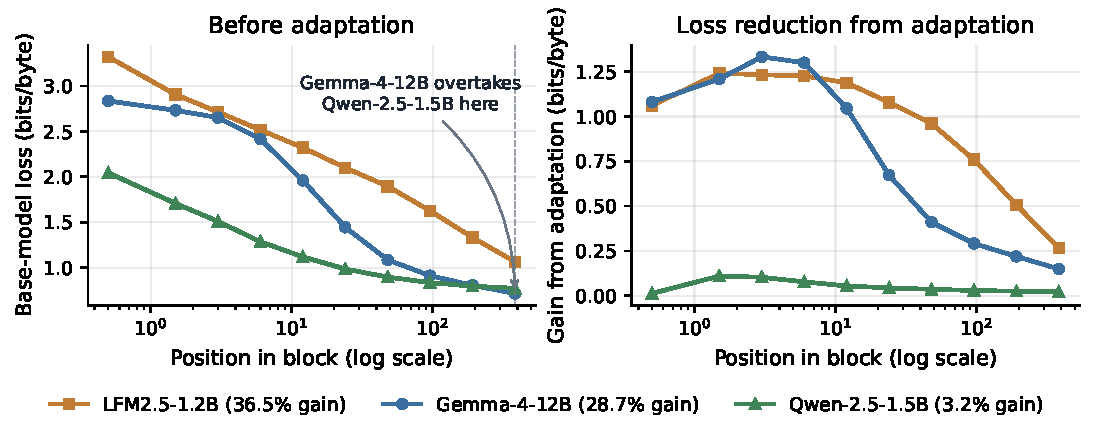
\includegraphics[width=0.8\columnwidth]{figures/fig_block_position.pdf}
\caption{\textbf{Why the unadapted number mis-ranks: it is largely scoring cold starts.} Base loss
by position within a packed $512$-token evaluation block. Unadapted, Gemma-4-12B opens a block at
$2.83$ bits per byte against Qwen-2.5-1.5B's $2.04$---a 12B model losing to a 1.5B one---and closes
it at $0.72$ against $0.77$. A block average over-weights the opening, and that is \emph{part} of
what puts Gemma-4-12B ninth of eleven on zero-shot BPB (Table~\ref{tab:mechanism}): discarding the
opening outright recovers about a quarter of the gap between the two readings and no more
(Appendix~\ref{app:robust}). \emph{Right:} the loss reduction adaptation buys at each position is
largest in the opening but does not vanish after it---adaptation teaches the corpus's opening
conventions, and does more besides.}
\label{fig:blockpos}
\end{figure}
\subsection{The same comparison on four independent yardsticks}
\label{sec:coverage}
One criterion is one opinion. Table~\ref{tab:coverage} runs the entire comparison four times, each
corpus judged only against a criterion built from its own held-out text: news, Reddit, Hacker
News and arXiv mathematics. Two patterns hold across all four domains and both scoring conventions:
adapted BPB never falls below a public benchmark in any row, and no public benchmark reaches the top
of any row. Against every selector, size included, it leads or ties five of the eight. On news and Reddit both generative suites sit far
below chance by point estimate---$0.182$ on the news criterion, picking the worse model four times
out of five---while on Hacker News MMLU-Pro reaches $0.727$ and on mathematics both recover to
$0.700$--$0.800$.

Ranking by size scores higher in three of the rows---news strict and both Hacker News rows, at
$0.818$, $1.000$ and $0.818$. Size is a strong baseline, and adapted BPB still beats it across the full
range of all $136$ pairs.

\begin{table}[t]
\centering\small
\resizebox{\textwidth}{!}{
\begin{tabular}{llcccccc}
\toprule
& & \textbf{Adapted} & \textbf{Zero-shot} & & & & \textbf{Param.} \\
\textbf{Criterion built from} & \textbf{scoring} & \textbf{BPB} & \textbf{BPB} & \textbf{HellaSwag} & \textbf{GSM8K} & \textbf{MMLU-Pro} & \textbf{count} \\
\midrule
Google News (11) & lenient & \textbf{0.909}$^\dagger$ & 0.545 & 0.818 & 0.182 & 0.182 & 0.636 \\
 & strict & 0.727 & 0.727 & 0.636 & 0.364 & 0.364 & \textbf{0.818} \\
\addlinespace
Reddit (11) & lenient & \textbf{1.000} & 0.636 & 0.909 & 0.273 & 0.273 & 0.727 \\
 & strict & \textbf{0.909} & 0.727 & 0.818 & 0.364 & 0.364 & 0.818 \\
\addlinespace
Hacker News (10) & lenient & 0.900 & 0.800 & 0.800 & 0.500 & 0.600 & \textbf{1.000} \\
(11) & strict & 0.727 & \textbf{0.818} & 0.636 & 0.545 & 0.727 & \textbf{0.818} \\
\addlinespace
arXiv math (10) & lenient & \textbf{0.900} & \textbf{0.900} & 0.600 & 0.700 & 0.700 & 0.800 \\
 & strict & \textbf{1.000} & \textbf{1.000} & 0.600 & 0.800 & 0.800 & 0.800 \\

\bottomrule
\end{tabular}
}
\caption{\textbf{The same comparison, run four times against four independent yardsticks.}
\emph{Eleven-model cohort; $10$--$11$ size-matched pairs per corpus.} Each row block scores every selector against a criterion built from \emph{that} corpus's own held-out text---post-release for
Reddit, Hacker News and arXiv, screened rather than post-dated for news
(Section~\ref{sec:criterion})---over the size-matched pairs (count in parentheses; Hacker News has
ten under lenient scoring and eleven under strict, because a pair the criterion ties orders
nothing). Bold is the leader in the row;
$\dagger$ marks an interval clearing chance. Two things replicate across all four domains and both
conventions: adapted BPB never falls below a public benchmark in any row, and no public benchmark
reaches the top of any row; against every selector it leads or ties five of the eight. It holds the highest point
estimate on two of the four corpora under both conventions---outright on Reddit, tied with the
unadapted reading on arXiv---while ranking by size leads three rows. At ten or eleven pairs per
corpus almost no cell here has the power to clear chance---one of the
forty-eight does---so this table is read for its orderings, not its intervals. GSM8K and MMLU-Pro
fall as low as $0.182$.}
\label{tab:coverage}
\end{table}
\subsection{What it changes}
\label{sec:divergence}
Aggregates hide the thing a practitioner wants to see: which model does this actually change (Table~\ref{tab:regret} prices each choice)?
Gemma-4-12B is the case to look at. Among the eleven models of Table~\ref{tab:static} it is second
by adapted BPB, second by the in-domain criterion, and \emph{seventh} on both MMLU-Pro and GSM8K. A team reading the scorecard would not shortlist it. Scorecard gaps are also wildly out of scale with what they decide, as the fine-tune below shows.

\begin{figure}[t]
\centering
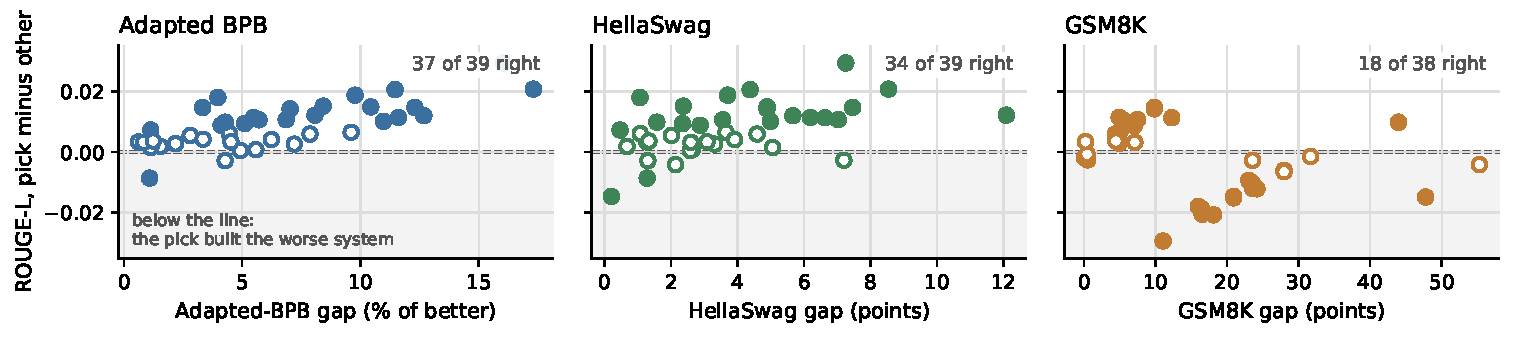
\includegraphics[width=\textwidth]{figures/fig_downstream.pdf}
\caption{\textbf{Did the selector's pick build the better system?} Every size-matched pair of the
fifteen fine-tuned models, oriented so the selector prefers the first: $x$ is how strongly it
prefers it, $y$ how much better that model's fine-tuned system scored. Above the line is a pair the
selector got right; filled markers are pairs the fine-tune itself resolves. Adapted BPB is right on
$37$ of the $39$ pairs, and on $21$ of the $22$ the fine-tune separates; HellaSwag follows at
$34$. GSM8K is right on $18$ of $38$, and every one of its eleven gaps between $15$ and $25$ points
sits \emph{below} the line, on a pair where it picked the worse system.}
\label{fig:downstream}
\end{figure}
\paragraph{So we fine-tuned them.} Every criterion so far lives in the corpus the selector adapted
on, so we left it. We fine-tuned fifteen of the seventeen models---every one that fits
a single GPU---on a real in-domain task, writing the opening paragraph of a news article from its
body, with one identical LoRA recipe and ROUGE-L against the human-written lede on $500$ held-out
articles from a split neither the criterion nor the BPB test blocks touch. The analysis was fixed
in code before the jobs ran (Appendix~\ref{sec:downstream}).

Scored against the fine-tuned systems over all $39$ size-matched pairs they form, the headline
repeats on an outcome nothing here was tuned against. Adapted BPB orders $0.949$ of the pairs
correctly, $[0.817, 1.000]$, ahead of HellaSwag at $0.872$, while GSM8K and MMLU-Pro sit at $0.474$
and $0.513$---a coin (Figure~\ref{fig:downstream}, Table~\ref{tab:downstream}). Its lead over
parameter count is statistically resolved under this recipe, $+0.231$ $[+0.059, +0.452]$, and on the
pairs the fine-tune
itself separates it picks the better system in $21$ of the $22$. A deliberately different
recipe---four times the rank, three times the learning rate, half the batch, a new seed---leaves the
systems' ordering almost unchanged (Spearman $0.982$) and adapted BPB still first at $0.923$, right on
all $20$ pairs that recipe separates. Table~\ref{tab:outofbox} shows why this matters: a model's
benchmark standing is a poor guide to where it finishes, while adapted BPB places all fifteen within
one rank of their final order. \textbf{Gemma-4-12B}, $9$th and $8$th of
fifteen on GSM8K and MMLU-Pro, builds the best system of the fifteen, beating Ministral-3-14B by $+0.018$ $[+0.011, +0.025]$; and the
$55.3$-point GSM8K gap between Llama-3.2-1B and Qwen-2.5-1.5B buys no measurable difference once both
are fine-tuned. Every model improved on its own base weights and cleared what copying the article's
first sentence scores ($0.125$).
\begin{table}[t]
\centering\small
\begin{tabular}{lccccc}
\toprule
& \multicolumn{3}{c}{\textbf{Out of the box}} & \textbf{After} & \textbf{Adapted BPB} \\
\cmidrule(lr){2-4}
\textbf{Model} & raw loss & GSM8K & MMLU-Pro & \textbf{fine-tuning} & \textbf{predicted} \\
\midrule
Gemma-4-12B  & 13 & \phantom{0}9 & \phantom{0}8 & \textbf{\phantom{0}1} & \phantom{0}2 \\
Llama-3.2-1B & 10 & 15 & 15 & \textbf{11} & 11 \\
LFM2.5-1.2B  & 15 & 12 & 13 & \textbf{14} & 14 \\
\bottomrule
\end{tabular}
\caption{\textbf{How a model looks is not how it finishes.} Rank among the fifteen fine-tuned models
($1$ is best). The benchmarks misjudge where these models end up, and raw loss misjudges
Gemma-4-12B by twelve places: it is mid-table on both benchmarks and near the bottom on raw loss,
then builds the best system of all. Llama-3.2-1B is last on both benchmarks and finishes eleventh.
Adapted BPB, measured before any task fine-tuning, places every model within a single rank of where
it finishes---all fifteen, and eleven exactly.}
\label{tab:outofbox}
\end{table}
\section{Recommended Practice}
\label{sec:using}

\begin{enumerate}[leftmargin=*]\setlength\itemsep{2pt}
\item \textbf{When candidates differ by more than about $2\times$ in parameters, the larger one is
usually the better choice.} Size is a good rule of thumb there, though adapted BPB beats it even across
the full $70\times$ range; the protocol is built for the case where size has stopped deciding.
\item \textbf{The corpus should come from the target domain, or close to it}, dated after every
candidate shipped and screened as in Section~\ref{sec:protocol}. Nearby text can work
as well: on the ten pairs we tested, Reddit BPB predicted the news fine-tune as well as news BPB did
(Appendix~\ref{sec:downstream}). The choice of corpus determines what the
ranking tracks, so it should match the capability that matters.
\item \textbf{Every finalist is adapted under one identical budget and ranked by adapted BPB}, at the cost
in GPU-minutes given on page~\pageref{fig:selectors}: cheap enough to run on every candidate rather
than a shortlist.
\item \textbf{The unadapted number is best read as a free screen, not the selector.} A candidate
badly off-distribution for the target text shows up in it, but on its own it reaches only $0.545$ against the
in-domain criterion in the size-matched band under lenient scoring, with an interval spanning
chance; under strict the two readings are level, so this is the one place adaptation may buy
nothing.
\item \textbf{With two or three candidates rather than a cohort, the \emph{gap} is what matters, and
we recommend treating anything under $2\%$ as a tie.} Two floors say what a gap must clear: re-running the \emph{same} model on a different seed
moved adapted BPB by up to $1.24\%$ (Gemma-4-12B; the median model, $0.01\%$), and token-aligned
blocks add up to $0.18\%$ (Appendix~\ref{app:robust}); the worst case, rounded up, is $2\%$. Above it: of
the $33$ size-matched pairs at least $2\%$ apart, the lower-BPB model was the criterion's preference
in \textbf{all $33$} lenient and $30$ of $33$ strict. Closer than that, the choice is better made on
licence, latency or serving cost. The threshold was chosen after seeing this cohort, so
Table~\ref{tab:decision} is best read as a calibration rather than an estimate.
\end{enumerate}
Results are comparable only when corpus revision, split, context length, marker masking, adaptation
configuration and update budget all match; changing any of them creates a new benchmark rather than a
new measurement of the old one.

\section{Conclusion}
Public benchmarks were built to compare models in general, and that makes them an unreliable guide to
the narrower question most teams face: which base model will serve a particular domain best. This work
shows that a cheap measurement answers that question better. Adapting every candidate to recent
in-domain text under one identical, small budget and ranking by bits per byte selected the better
model at least as often as any public benchmark across four corpora, resolved its lead over parameter
count under lenient scoring, and predicted the quality of fifteen real fine-tuned systems, placing
each within one rank of its final position.

\paragraph{Why it matters.} The measurement is tokenizer-agnostic, costs minutes of GPU time per
candidate, and is computed on text the evaluator controls, so it cannot be prepared for in advance and
can be rerun whenever a new model appears. It also captures what a benchmark structurally cannot: how
good a model becomes once adapted, which is the quantity a deployment depends on. For research it
offers a contamination-resistant complement to public leaderboards, and a way to compare models that
does not rest on any fixed exam.

\paragraph{Anticipated objections.} Four concerns arise naturally, and each was tested directly.
\emph{Circularity}---that a yardstick built from the same corpus rewards the method---is answered by
fine-tuning the models and scoring the resulting systems on separate documents against human-written
references; that ranking agrees with the criterion at Spearman $0.921$. \emph{Recipe
dependence}---that the downstream agreement reflects the adaptation recipe---is answered by repeating
every fine-tune with a substantially different recipe, which leaves the ranking nearly unchanged
(Spearman $0.982$). \emph{Contamination} is addressed with text dated after the models' release or
screened for membership, and \emph{selection bias} by scoring every size-matched pair under
preregistered rules. The main open question is statistical power: with seventeen models the lead over
HellaSwag is consistent but not yet resolved, and a larger, more diverse cohort is the natural next
step.
{\small
\bibliographystyle{plain}
\begin{multicols}{2}
\begin{thebibliography}{99}
\setlength{\itemsep}{0pt}
\bibitem{shannon1951prediction} Shannon, C. E. (1951). Prediction and entropy of printed English. Bell System Technical Journal, 30:50--64.
\bibitem{mielke2019perplexity} Mielke, S. J. (2019). Can you compare perplexity across different segmentations? Technical note.
\bibitem{gao2020pile} Gao, L., et al. (2021). The Pile: An 800GB Dataset of Diverse Text for Language Modeling. arXiv:2101.00027.
\bibitem{ahia2023languages} Ahia, O., et al. (2023). Do All Languages Cost the Same? Tokenization in the Era of Commercial Language Models. EMNLP. arXiv:2305.13707.
\bibitem{magnusson2023paloma} Magnusson, I., et al. (2023). Paloma: A Benchmark for Evaluating Language Model Fit. arXiv:2312.10523.
\bibitem{carlini2021extracting} Carlini, N., et al. (2021). Extracting Training Data from Large Language Models. USENIX Security.
\bibitem{carlini2022quantifying} Carlini, N., et al. (2022). Quantifying Memorization Across Neural Language Models. ICLR 2023. arXiv:2202.07646.
\bibitem{lee2022deduplicating} Lee, K., et al. (2022). Deduplicating Training Data Makes Language Models Better. ACL. arXiv:2107.06499.
\bibitem{shi2023mink} Shi, W., et al. (2023). Detecting Pretraining Data from Large Language Models. ICLR 2024. arXiv:2310.16789.
\bibitem{zhang2024minkpp} Zhang, J., et al. (2024). Min-K\%++: Improved Baseline for Detecting Pre-Training Data from Large Language Models. ICLR 2025. arXiv:2404.02936.
\bibitem{xu2024survey} Xu, C., et al. (2024). Benchmark Data Contamination of Large Language Models: A Survey. arXiv:2406.04244.
\bibitem{gao2024lmeval} Gao, L., Biderman, S., et al. (2024). A Framework for Few-Shot Language Model Evaluation (lm-evaluation-harness). EleutherAI.
\bibitem{heineman2025signal} Heineman, D., Hofmann, V., Magnusson, I., et al. (2025). Signal and Noise: A Framework for Reducing Uncertainty in Language Model Evaluation. NeurIPS 2025.
\bibitem{thrush2024perplexity} Thrush, T., Potts, C., and Hashimoto, T. (2024). Improving Pretraining Data Using Perplexity Correlations. arXiv:2409.05816.

\bibitem{zhang2025trainbeforetest} Zhang, G., Dominguez-Olmedo, R., and Hardt, M. (2025). Train-before-Test Harmonizes Language Model Rankings. arXiv:2507.05195.
\bibitem{ruan2024observational} Ruan, Y., Maddison, C. J., and Hashimoto, T. (2024). Observational Scaling Laws and the Predictability of Language Model Performance. NeurIPS 2024.
\bibitem{gadre2025scales} Gadre, S. Y., Smyrnis, G., Shankar, V., et al. (2025). Language Models Scale Reliably with Over-Training and on Downstream Tasks. ICLR 2025.
\bibitem{wang2024mmlupro} Wang, Y., et al. (2024). MMLU-Pro: A More Robust and Challenging Multi-Task Language Understanding Benchmark. NeurIPS D\&B. arXiv:2406.01574.
\bibitem{zellers2019hellaswag} Zellers, R., et al. (2019). HellaSwag: Can a Machine Really Finish Your Sentence? ACL. arXiv:1905.07830.
\bibitem{cobbe2021gsm8k} Cobbe, K., et al. (2021). Training Verifiers to Solve Math Word Problems (GSM8K). arXiv:2110.14168.
\bibitem{krause2018dynamic} Krause, B., Kahembwe, E., Murray, I., and Renals, S. (2018). Dynamic Evaluation of Neural Sequence Models. ICML 2018. arXiv:1709.07432.
\bibitem{krause2019dynamictransformer} Krause, B., Kahembwe, E., Murray, I., and Renals, S. (2019). Dynamic Evaluation of Transformer Language Models. arXiv:1904.08378.
\bibitem{gururangan2020dapt} Gururangan, S., et al. (2020). Don't Stop Pretraining: Adapt Language Models to Domains and Tasks. ACL. arXiv:2004.10964.
\bibitem{hu2021lora} Hu, E. J., et al. (2021). LoRA: Low-Rank Adaptation of Large Language Models. ICLR 2022. arXiv:2106.09685.
\bibitem{dubey2024llama3} Dubey, A., et al. (2024). The Llama 3 Herd of Models. arXiv:2407.21783.
\bibitem{yang2024qwen25} Yang, A., et al. (2024). Qwen2.5 Technical Report. arXiv:2412.15115.
\bibitem{gemma2026gemma4} Gemma Team (2026). Gemma 4 Technical Report. arXiv:2607.02770.
\bibitem{liu2026ministral3} Liu, A. H., et al. (2026). Ministral 3. arXiv:2601.08584.
\bibitem{qwen2026qwen35} Qwen Team (2026). Qwen3.5: Towards Native Multimodal Agents.
Official release and model card. \url{https://qwen.ai/blog?id=qwen3.5}.
\end{thebibliography}
\end{multicols}
}
\appendix
\small

\section{Related Work}
\label{sec:related}
\textbf{From perplexity to comparable loss.} Language modelling was grounded in byte- and
character-level entropy from the start \cite{shannon1951prediction}, but token-level perplexity
depends on each model's vocabulary \cite{mielke2019perplexity,ahia2023languages}; normalising by
UTF-8 bytes restores a common unit \cite{gao2020pile,magnusson2023paloma}, and loss-based metrics
carry better signal and lower noise than accuracy across 465 models \cite{heineman2025signal}. Our
contribution is the operational protocol around the metric, not the metric.

\textbf{Where the loss is measured matters.} Thrush et al.\ turn the varying correlation between
per-domain perplexity and benchmark performance into a pretraining-data selection rule
\cite{thrush2024perplexity}. Their estimand is the complement of ours: they fix the benchmark suite
and choose data to \emph{train} one strong model, where we fix the candidate pool and ask how the
\emph{selection ranking} moves.

\textbf{Equal preparation.} Dynamic evaluation updates a model on recent test history
\cite{krause2018dynamic,krause2019dynamictransformer} and domain-adaptive pretraining improves fit to
a target distribution \cite{gururangan2020dapt}. Closest to our motivation, \emph{train-before-test}
gives 61 models identical supervised preparation across 24 tasks and raises cross-benchmark Kendall
agreement from $0.52$ to $0.76$ \cite{zhang2025trainbeforetest}; they rank post-fine-tuning accuracy
on public labelled benchmarks, where we rank held-out fit after \emph{unsupervised} adaptation to a
fresh corpus, across tokenizers. The core idea---prepare every candidate identically before
comparing them---is theirs; what we add is doing it without labels, on text no vendor has seen, in a
unit that compares tokenizers, and checking the result against real fine-tuned systems. Controlled
families show a smooth loss-to-error relation
\cite{gadre2025scales,ruan2024observational}; we test it \emph{across} families.

\textbf{Contamination.} Models memorise duplicated pretraining text
\cite{carlini2021extracting,carlini2022quantifying}, so deduplication and contamination analysis are
necessary \cite{lee2022deduplicating,xu2024survey}; reference-free membership signals are useful
screens \cite{shi2023mink,zhang2024minkpp} but prove nothing about a proprietary training set, so we
use them only for conservative quarantine.
\begin{table}[ht]
\centering
\small
\resizebox{\columnwidth}{!}{
\begin{tabular}{lrrrrl}
\toprule
\textbf{Corpus} & \textbf{Raw records} & \textbf{Documents} & \textbf{Median words} & \textbf{Text} & \textbf{Contamination control} \\
\midrule
Google News, 8 Jun 2026     & \phantom{0,0}119{,}054 & 119{,}054 & 362 & 361\,MB & Min-K++ / context / perturbation union \\
Reddit, 6--10 Aug 2026$^{\dagger}$ & 3{,}054{,}623 & 141{,}527 & 624 & 533\,MB & Post-release scrape \\
Hacker News, 6--10 Aug 2026 & \phantom{0,0}\phantom{0}60{,}814 & \phantom{00}6{,}086 & 690 & \phantom{0}46\,MB & Post-release scrape \\
arXiv \texttt{math.*}, 9 Jun--20 Aug 2026$^{\ddagger}$ & \phantom{0,00}\phantom{0}3{,}207 & \phantom{00}3{,}207 & --- & \phantom{0}15\,MB & Post-release scrape $+$ GSM8K shingle screen \\
\bottomrule
\end{tabular}
}
\caption{Corpora. All four receive identical exact-deduplication, Gopher quality filtering and
MinHash/LSH near-duplicate removal at Jaccard $0.60$; they differ in \emph{contamination} control,
deliberately. The reference-free screen ran on the news corpus, whose 8 June 2026 snapshot predates
part of the cohort's release window; Reddit and Hacker News were scraped after every model shipped,
as was most of the arXiv set, and they are
protected by construction. Reddit and Hacker News comments are grouped to document length.
$^{\dagger}$Four days are available in the stated range. $^{\ddagger}$Used only for the mathematics
adaptation.}
\label{tab:corpora}
\end{table}
\section{The Criterion: Construction and Composition}
\label{app:criterion}
Table~\ref{tab:criterion} gives the four criteria. Items come from each corpus's own held-out test
split, reproduced with the evaluation pipeline's shuffle and seed. Each hides one entity or number
span and supplies $1{,}200$ characters of preceding context; spans occurring earlier in the prompt
are dropped, so retrieval from context cannot substitute for prediction. Generation is greedy, scored
by string match, and produced by the released base weights.

Composition differs across the four, which is why we never compare their levels: news is
entity-dominated and Reddit number-dominated, and numeric spans are simply easier---answered at
$0.279$ and $0.325$ against $0.180$ and $0.060$ for entity spans on those two corpora. Within a
corpus every selector is scored on identical items, which is the only comparison the paper draws.

A worked item, answered by two of the cohort:

\begin{center}\small
\fbox{\parbox{0.94\columnwidth}{\ldots\ MBDA is owned by Airbus ($37.5\%$), BAE Systems ($37.5\%$), and Leonardo
(\underline{\hspace{2em}}\\[2pt]
\emph{hidden span:} \texttt{25\%}\quad
\emph{Gemma-4-12B:} \texttt{25\%).} \checkmark\quad
\emph{Qwen-2.5-0.5B:} \texttt{30\%).} $\times$}}
\end{center}

\noindent The answer is nowhere in the context; the model has to know the company, or
do the sum.

\paragraph{How precisely is the quiz known?} We resample its $2{,}500$ items, paired across models
so that item difficulty cancels out of a between-model difference. It separates the cohort from
$0.066$ to $0.213$ and resolves seven of the ten adjacent pairs under lenient scoring, two under
strict; Table~\ref{tab:mechanism} carries every interval. Adjacent models it cannot order are
reported as unordered rather than counted as some selector's mistake.

\paragraph{Does sharing text with BPB make it circular?} The criterion and the BPB evaluation
do come from the same held-out bytes. The evidence that this
does not drive the result is internal: the reading \emph{mechanically closest} to the
criterion---zero-shot BPB, same weights, same text, same conditional---is the weaker of the two at
$0.545$, while the adapted reading, from different weights, is the best. Shared bytes alone do not
buy agreement, and Section~\ref{sec:divergence} leaves the loop altogether: a real fine-tune, scored
on different documents against a human-written reference.

\paragraph{Is it just measuring size?} Such a criterion could also be a size proxy. Over the full $70\times$ range it does track size
($\rho = 0.918$ against log parameters), as any capability measure should. \emph{Inside} the band,
parameter count clears chance against none of the four per-corpus criteria, though it does on the
extended news cohort under strict ($0.750$ $[0.517, 0.932]$), and two dense size inversions
resolve---Gemma-4-12B over the larger Ministral-3-14B, $+0.044$ $[+0.032, +0.057]$, and Llama-3.2-1B
over Qwen-2.5-1.5B, $+0.016$ $[+0.006, +0.026]$. (The one mixture-of-experts model
activates $3$B of $34.7$B and is never used as a size example.)

\paragraph{Screening.} The news corpus additionally passes three reference-free membership screens
per model---Min-K++ (normalised likelihood of the lowest-probability $K{=}20\%$ target tokens),
context sensitivity (target NLL with and without sampled same-corpus prefixes), and, for flagged
candidates only, preference over two word-swap/placeholder perturbations. The global union
quarantined $80$ unique sequences, after which every model receives the identical retained corpus.
Near-$100\%$ preference for the unperturbed original is expected---fluency alone produces it---so we
draw no memorisation conclusion from it (\texttt{results/contamination/}).
\begin{table}[ht]
\centering\small
\begin{tabular}{lrrrl}
\toprule
\textbf{Criterion} & \textbf{Items} & \textbf{Entity} & \textbf{Number} & \textbf{Drawn from} \\
\midrule
Google News, 8 Jun 2026        & 2{,}500 & 1{,}677 & \phantom{0}823 & test split of a $119{,}054$-doc corpus \\
Reddit, 6--10 Aug 2026         & 2{,}500 & \phantom{0}900 & 1{,}600 & test split of a $141{,}527$-doc corpus \\
Hacker News, 6--10 Aug 2026    & 2{,}005 & \phantom{0}931 & 1{,}074 & test split of a \phantom{00}$6{,}086$-doc corpus \\
arXiv \texttt{math.*}, 2026    & 1{,}911 & \phantom{0}949 & \phantom{0}962 & test split of a \phantom{00}$3{,}207$-doc corpus \\
\bottomrule
\end{tabular}
\caption{The four criteria. Composition differs by corpus and that is why their \emph{levels} are not
comparable across rows: news is entity-dominated, Reddit number-dominated. Within a corpus the
comparison is between selectors on identical items, which is the only comparison we make. The
mathematics set is the thinnest, drawing on $320$ held-out documents with up to eight spans from
each.}
\label{tab:criterion}
\end{table}

\section{The Full Benchmark Alignment}
\label{app:alignment}
Table~\ref{tab:alignment} reports all twenty-four (corpus $\times$ reading $\times$ benchmark) cells
over the full $55$ pairs; Table~\ref{tab:regret} prices each reading's top-1 pick against each
benchmark's own.  The rotation (Appendix~\ref{app:robust}) is legible column by column: adapting on general
text raises HellaSwag agreement and lowers the GSM8K column on every corpus and MMLU-Pro on two of
the three general-text corpora; adapting on mathematics reverses the GSM8K half. The pairs-correct column---GSM8K only---shows how little of this is visible in a rank
correlation: across its eight rows it spans $41/55$ to $49/55$.
\begin{table}[t]
\centering\small
\begin{tabular}{llcccc}
\toprule
& & \multicolumn{3}{c}{\textbf{Rank correlation ($\rho$) with}} & \textbf{GSM8K pairs} \\
\cmidrule(lr){3-5}
\textbf{Corpus} & \textbf{Reading} & GSM8K & MMLU-Pro & HellaSwag & \textbf{correct} \\
\midrule
% generated by tools/analyze_alignment_matrix.py
News & zero-shot & 0.800 & 0.845 & 0.718 & 45 & 45 & 44 \\
 & adapted & 0.700 & 0.773 & 0.982 & 42 & 44 & 53 \\
\addlinespace
Reddit & zero-shot & 0.745 & 0.782 & 0.655 & 43 & 43 & 42 \\
 & adapted & 0.655 & 0.745 & 0.964 & 41 & 43 & 52 \\
\addlinespace
Hacker News & zero-shot & 0.800 & 0.809 & 0.627 & 44 & 44 & 43 \\
 & adapted & 0.745 & 0.855 & 0.973 & 44 & 46 & 53 \\
\addlinespace
Math (arXiv) & zero-shot & 0.764 & 0.736 & 0.482 & 43 & 43 & 40 \\
 & adapted & 0.909 & 0.927 & 0.818 & 49 & 49 & 46 \\

\bottomrule
\end{tabular}
\caption{\emph{Eleven-model cohort, all $55$ pairs (no size band).} All twenty-four (corpus
$\times$ reading $\times$ benchmark) cells, recomputed from the committed cells. The rotation is visible column by column: adapting on general
text raises HellaSwag agreement and lowers GSM8K everywhere, while adapting on mathematics
reverses it.}
\label{tab:alignment}
\end{table}
\begin{table}[t]
\centering\small
\begin{tabular}{llccc}
\toprule
& & \multicolumn{3}{c}{\textbf{Accuracy given up vs.\ the benchmark's own pick (pts)}} \\
\cmidrule(lr){3-5}
\textbf{Corpus and reading} & \textbf{Picks} & GSM8K & MMLU-Pro & HellaSwag \\
\midrule
% generated by tools/analyze_alignment_matrix.py
News zero-shot & Qwen-3.5-35B-MoE & 0.0 & 0.0 & 2.4 \\
News adapted & Gemma-4-31B & 1.6 & 4.3 & 0.0 \\
Reddit zero-shot & Ministral-3-14B & 5.8 & 8.6 & 5.0 \\
Reddit adapted & Gemma-4-31B & 1.6 & 4.3 & 0.0 \\
Hacker News zero-shot & Qwen-3.5-35B-MoE & 0.0 & 0.0 & 2.4 \\
Hacker News adapted & Gemma-4-31B & 1.6 & 4.3 & 0.0 \\
Math (arXiv) zero-shot & Qwen-3.5-35B-MoE & 0.0 & 0.0 & 2.4 \\
Math (arXiv) adapted & Qwen-3.5-35B-MoE & 0.0 & 0.0 & 2.4 \\

\bottomrule
\end{tabular}
\caption{\textbf{What choosing on BPB costs you on each benchmark.} For every corpus and reading, the
model the ranking puts first and how many accuracy points that costs against each benchmark's own
top-1 model. Only three distinct picks occur in eight rows, which is itself the finding: the adapted
ranking selects Gemma-4-31B on every general-text corpus---the HellaSwag leader outright, at $1.6$
GSM8K and $4.3$ MMLU-Pro points---while adapting on mathematics recovers the GSM8K and MMLU-Pro
leader at zero regret. The corpus, not the metric, decides which column you pay in.}
\label{tab:regret}
\end{table}
\begin{table}[t]
\centering\small
\begin{tabular}{lcccc}
\toprule
\textbf{Model} & \textbf{Adapted BPB} & \textbf{MMLU-Pro} & \textbf{HellaSwag} & \textbf{GSM8K} \\
\midrule
% generated by tools/analyze_static_benchmarks.py
Gemma-4-31B & \textbf{0.624 (1)} & 57.8 (2) & \textbf{87.9 (1)} & 84.2 (3) \\
Gemma-4-12B & 0.653 (2) & 44.7 (7) & 84.2 (3) & 63.6 (7) \\
Qwen-3.5-35B-MoE & 0.678 (3) & \textbf{62.0 (1)} & 85.5 (2) & \textbf{86.5 (1)} \\
Ministral-3-14B & 0.679 (4) & 54.1 (4) & 82.9 (4) & 80.7 (5) \\
Qwen-3.5-9B & 0.708 (5) & 56.2 (3) & 81.6 (5) & 86.0 (2) \\
Qwen-2.5-7B & 0.717 (6) & 47.5 (6) & 80.3 (6) & 81.3 (4) \\
Qwen-3.5-4B & 0.749 (7) & 52.5 (5) & 77.2 (7) & 80.4 (6) \\
Llama-3.2-1B & 0.771 (8) & 11.7 (11) & 65.8 (9) & 6.5 (11) \\
Qwen-2.5-1.5B & 0.797 (9) & 25.0 (8) & 67.8 (8) & 61.1 (8) \\
LiquidAI-LFM2.5 & 0.852 (10) & 15.5 (10) & 60.9 (10) & 55.0 (9) \\
Qwen-2.5-0.5B & 0.901 (11) & 16.7 (9) & 51.8 (11) & 34.7 (10) \\

\bottomrule
\end{tabular}
\caption{\textbf{Where the readings disagree, in one place.} \emph{Eleven-model cohort, news.}
Adapted news BPB (lower is better) beside the three benchmark scores, rank in parentheses. Gemma-4-12B is the case to look at: second by BPB,
third on HellaSwag, and \emph{seventh} on both MMLU-Pro and GSM8K---and second by the independent
in-domain criterion (Table~\ref{tab:mechanism}). Llama-3.2-1B and Qwen-2.5-1.5B are adjacent in BPB
and $2.1$ HellaSwag points apart, yet $55$ GSM8K points apart.}
\label{tab:static}
\end{table}

\begin{figure}[ht]
\centering
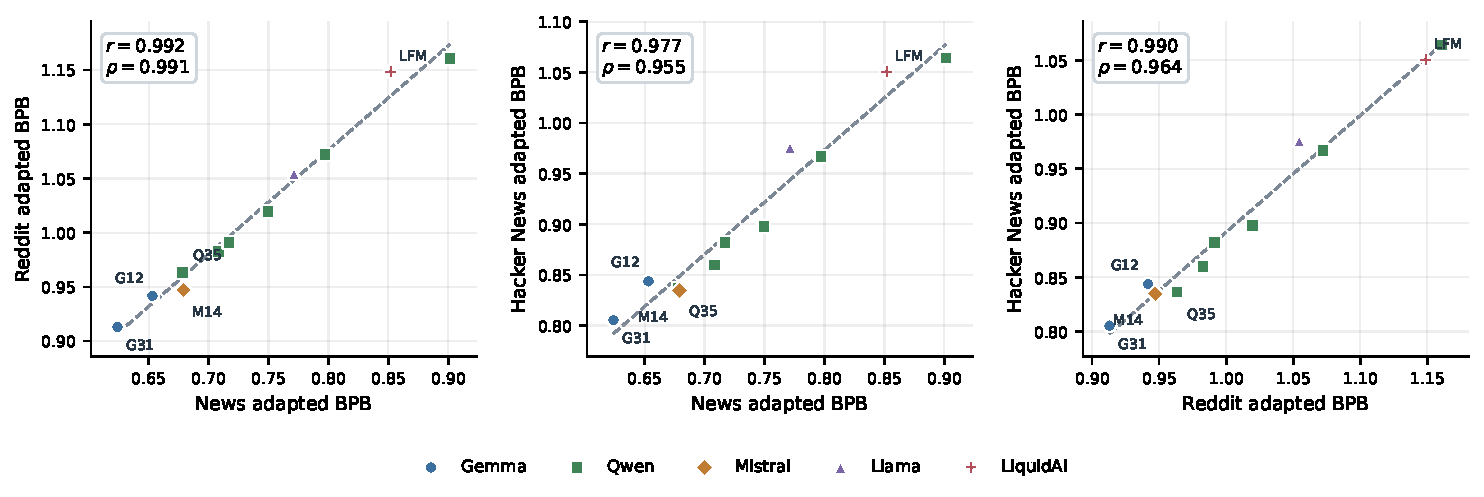
\includegraphics[width=\columnwidth]{figures/fig_cross_corpus.pdf}
\caption{Pairwise adapted-BPB agreement across domains. Absolute difficulty changes, but points
remain close to a monotone shared ordering: Pearson correlations between score values are $0.992$
(news--Reddit), $0.977$ (news--Hacker News) and $0.990$ (Reddit--Hacker News). G31/G12 denote Gemma-4-31B/12B; Q35 is
Qwen-3.5-35B-MoE; M14 is Ministral-3-14B.}
\label{fig:crosscorpus}
\end{figure}
\section{Robustness and Measurement Artefacts}
\label{app:robust}

\paragraph{Stability across domains.}\label{sec:domains} All eleven models ran on three independently collected domains under the same recipe
(Tables~\ref{tab:corpora} and~\ref{tab:leaderboard}). Adaptation genuinely changes the
choice---zero-shot and adapted rankings agree only at Spearman $\rho = 0.655$ on news, $0.609$ on
Reddit and $0.682$ on Hacker News, with models moving up to seven places---and the adapted ordering
then holds across domains: news and Reddit agree on nine of eleven exact ranks
($\rho = 0.991$, maximum displacement one), news against Hacker News gives $0.955$ and Reddit
against Hacker News $0.964$, and the agreement is not merely ordinal (Figure~\ref{fig:crosscorpus}).
\textbf{So does the zero-shot ordering}---$0.982$, $0.964$ and $0.973$ on the same three
comparisons. The tempting story is that adaptation buys stability, and
it does not; it buys a \emph{different} stable ordering, and Section~\ref{sec:mechanism} is the
evidence that it is the better of the two.

\paragraph{Why one shared configuration.} We first ran a per-model hyperparameter search and abandoned
it because its budget was confounded with model size: inside a fixed wall-clock allocation the two
largest models completed four trials each while the 1B models completed 17 and 18
(\texttt{results/legacy\_sweep/*/trials.csv}). That hands small models a better-tuned adapter and
biases the ranking by parameter count in a way no post-hoc correction can remove.

\paragraph{The cold start, seen a second way.} Varying the inference context on $64$ fixed held-out
target windows from $16$ to $2048$ tokens reproduces Figure~\ref{fig:blockpos}'s effect
non-positionally: both models improve with context and the larger improves faster, so any protocol
that scores short contexts under-rates the models that use long ones. Measured context sensitivity is
$0.032$ bits per byte per doubling, which is the constant the block-alignment bound below uses.

\paragraph{Token-aligned blocks: a real bias, bounded.} Evaluation blocks are 512 \emph{tokens}
rather than a fixed byte span, so models with different tokenizers score slightly different amounts
of text---5.92--6.24\,MB across the eleven-model cohort, a $5\%$ spread, and $9.9\%$ across the
seventeen. Bounding the resulting bias with the measured context sensitivity puts it at
$0.08\times$ the smallest adjacent rank gap in the eleven-model cohort. In the extended cohort the
bound is looser and worth stating: on the worst adjacent pair, Qwen2.5-3B over Falcon3-7B, whose BPB
gap is only $0.29\%$, the bound reaches $0.61\times$ the gap. It still \textbf{overturns no rank},
but byte-aligned blocking would remove the question, and we recommend it for future work.

\paragraph{The resolved comparison is not an artifact of a lucky seed.} Every adaptation cell ran
with the \texttt{torch} RNG unseeded, and the cluster bootstrap resamples models, so it carries no
within-cell training variance. A preregistered check---three seed replicates for all $17$ models,
$51$ cells, news corpus, everything else pinned---is confirmatory on all four questions it asked.
Median within-model SD of adapted BPB is $0.000087$ against a between-model SD of $0.074340$, a
ratio of $0.0012$; in-band pairwise accuracy is $0.900$ under each seed; \emph{no} in-band
pair---$0$ of $40$---reverses its ordering; and adding a seed-resampling stage moves the resolved
interval by $0.001$. The spread is not uniform: Gemma-4-12B is the one model where seed noise is
visible at all (SD $0.00315$, $5.3\times$ the next-largest spread).

\paragraph{Steering: direction, not magnitude.} Adapting on general text raises agreement with
HellaSwag on news from $\rho = 0.718$ to $0.982$ while GSM8K falls from $0.800$ to $0.700$ and
MMLU-Pro from $0.845$ to $0.773$; adapting on contamination-screened arXiv mathematics instead
raises GSM8K agreement to $0.909$ and restores the GSM8K oracle pick at zero regret,
while three general-text corpora tried as controls all leave GSM8K at or below the do-nothing
baseline. That is the rotation, and it is why the body reports only its direction. Because the
steering hypothesis predicts a
\emph{joint} movement, the better-powered statistic is a difference in differences---(GSM8K minus
HellaSwag selection accuracy under mathematics adaptation) minus the same quantity under a
general-text corpus---which is $+0.242$ pooled. Resampling models gives a strictly positive
difference in $93.7\%$ of draws; the stricter publisher-family clustering the mechanism itself
implies gives $80.9\%$ with not one negative draw in $20{,}000$, but no longer clears $0.05$ on any
tie convention. A leave-one-family-out jackknife shows why: dropping the two Gemma models takes the
pooled difference from $+0.242$ to $+0.056$. The remedy is more \emph{families}, not more models.

\paragraph{Discarding the cold start: how much does it buy?} (E10.) Each model was re-scored
zero-shot with per-token loss accumulated separately at every position in the $512$-token block, so
every cutoff $K$ is derivable from one pass; the falsifying outcome was fixed in advance---if any $K$
brought the free reading within one in-band pair of adapted BPB, the mechanism claim above would
have been withdrawn. It does not. Under lenient scoring in-band accuracy rises from $0.545$ at
$K{=}0$ to $0.636$ at $K{=}128$ and no further, closing $25\%$ of the $0.364$ gap to adapted BPB.
Under strict scoring the test is \emph{uninformative} and we say so rather than counting it: the two
readings already tie at $0.727$ there, so there is no gap for the cold start to be accused of
causing, and discarding positions only makes the free reading worse ($0.636$ at $K{\geq}128$). The
re-measured cells are not the published ones---they run up to $1.5\%$ low---so every cutoff is
compared against this run's \emph{own} $K{=}0$, which reproduces the published zero-shot selector
exactly under both conventions.

\begin{table}[ht]
\centering\small
\begin{tabular}{llrcrc}
\toprule
& & \multicolumn{2}{c}{\textbf{All in-band pairs}} & \multicolumn{2}{c}{\textbf{Criterion-resolved only}} \\
\cmidrule(lr){3-4}\cmidrule(lr){5-6}
\textbf{Scoring} & \textbf{Relative BPB gap} & pairs & agreement & pairs & agreement \\
\midrule
lenient & all & 40 & 0.900 & 35 & 0.971 \\
 & $\geq1\%$ & 38 & 0.947 & 35 & 0.971 \\
 & $\geq2\%$ & 33 & 1.000 & 32 & 1.000 \\
 & $\geq5\%$ & 22 & 1.000 & 22 & 1.000 \\
\midrule
strict & all & 40 & 0.850 & 31 & 0.968 \\
 & $\geq1\%$ & 38 & 0.895 & 31 & 0.968 \\
 & $\geq2\%$ & 33 & 0.909 & 28 & 0.964 \\
 & $\geq5\%$ & 22 & 0.955 & 19 & 1.000 \\

\bottomrule
\end{tabular}
\caption{\textbf{How often the lower adapted-BPB model is the better model, by how far apart they
are.} \emph{Extended cohort: 17 models, $40$ size-matched pairs.} Gaps are a percentage of the smaller adapted BPB. The measurement's own floor is about
$1.4\%$ (seed variation plus block alignment); Section~\ref{sec:using} rounds its rule up to the
$2\%$ row, where these counts begin.}
\label{tab:decision}
\end{table}
\paragraph{Three reproduction controls.} Re-running two Ministral-3-14B cells weeks later on
different hardware reproduced zero-shot BPB exactly and adapted BPB to within $0.0003$, two orders of
magnitude below the differences compared. Because the extension models were adapted on a different
software stack, a published cell (Qwen2.5-7B) was re-run through the extension pipeline; the analysis
refuses to pool the cohorts unless it reproduces within $1\%$, and it reproduces to $0.01\%$ on
adapted BPB ($0.7169$ against $0.7170$). And because benchmark rankings are themselves estimates,
recomputing selection accuracy while discarding pairs whose benchmark gap is smaller than $k$
combined standard errors leaves the result intact and slightly improves it: on GSM8K $0.909$ at
$k{=}0$ becomes $0.933$ at $k{=}3$, and on HellaSwag $0.836$ becomes $0.863$, so the metric's errors
concentrate in pairs the benchmark itself cannot separate.

\section{The Downstream Fine-Tune}
\label{sec:downstream}
Section~\ref{sec:divergence} reports the result; this is how it was built, and what it does and
does not license. It ran in two stages, each preregistered in code before its job returned: first the
two pairs on which the selectors disagree most (Gemma-4-12B against Ministral-3-14B, Llama-3.2-1B
against Qwen-2.5-1.5B), then every cohort model that fits one GPU, so that no pair is chosen by
anyone. Gemma-4-31B and Qwen-3.5-35B-MoE need more than one GPU \emph{for this fine-tune}---its
$1{,}280$-token sequences and its generation pass cost far more memory than the $512$-token
adaptation priced in Section~\ref{sec:intro}---and are excluded by that rule, which costs one in-band
pair of forty.

\paragraph{The task.} Journalistic convention makes a news article's first paragraph a standalone
summary of it, so the corpus supplies its own supervision: the input is the article with its opening
paragraph removed, truncated to $3{,}000$ characters, and the target is that paragraph. Articles
qualify if they have at least three paragraphs, an opening paragraph of $200$--$700$ characters
ending in sentence punctuation, and at least $800$ characters of remaining body. Of the $11{,}905$
validation documents, $3{,}627$ qualify; $2{,}000$ are sampled for training and $500$ for evaluation
under a fixed seed.

\paragraph{Why the validation split.} The in-domain criterion (Section~\ref{sec:criterion}) and the
BPB test blocks both live in the \emph{test} split. That is verified rather than assumed: the shipped
criterion items reproduce item-for-item from an independent reconstruction of the test split, and the
adaptation pipeline's contamination pass---which would have split the corpus differently---is off by
default and recorded as off in every published cell. Evaluation documents are then hashed against the
test documents twice, on full normalised text and on a $400$-character opening, the second because a
syndicated wire story is republished with an edited body and an identical lede. Four articles were
dropped by that second check and none by the first.

\paragraph{Equal preparation.} Both members of a pair get the paper's own adaptation recipe unchanged
---LoRA rank $16$, $\alpha{=}32$, dropout $0.05$, learning rate $10^{-4}$, effective batch $32$, $250$
steps---with prompt tokens masked out of the loss so the model is trained to write the lede rather
than to reconstruct the article. Nothing is tuned on either model, because a per-model search is
exactly the cost this protocol exists to avoid. The tokenizers differ, so the budget is matched in
update steps $\times$ batch $\times$ sequence length; each model's realised token count is in the
artifact. Decoding is greedy with a $180$-token cap and each checkpoint's own generation
configuration otherwise untouched, following Appendix~\ref{app:rescore}. The prompt is assembled
so that the instruction always survives truncation: the \emph{body} is cut to fit, never the
instruction after it, because right-truncating the assembled prompt would delete the instruction from
the longest articles at a different article count for each tokenizer---an asymmetry between the two
models being compared. At most four of the $500$ evaluation articles were cut for any model, and
none for three of them.

\paragraph{The decision rules, fixed before each run.} For the two chosen pairs: mean ROUGE-L F1
over the $500$ held-out articles, a paired bootstrap over articles ($20{,}000$ draws, $95\%$ percentile
interval) and a practical-equivalence margin of $0.01$---an interval excluding zero resolves the pair
for whichever reading predicted that winner. The first pair resolved for adapted BPB; the second was
inconclusive. For the full cohort: the fine-tuned ROUGE-L is treated as the criterion and every
selector is scored with the paper's own statistic---pairwise accuracy within $2\times$, model-level
cluster bootstrap, $20{,}000$ draws (Table~\ref{tab:downstream}). A separate guard voids any
comparison in which fine-tuning failed to improve a model over its own base weights, since ordering
unmoved models would order their base behaviour under another name. It did not fire: all fifteen
models gained between $+0.041$ and $+0.153$.

\paragraph{A second recipe.} Both readers of an earlier draft raised the same objection: the
fine-tune reused the selector's own recipe, so a model that adapts quickly under it could win both.
Recipe B changes every setting the two shared---LoRA rank $64$, $\alpha{=}128$, learning rate
$3\times10^{-4}$, effective batch $16$, $400$ steps, a new seed---on the same task, data, decoding and
metric, preregistered before it ran. It fits the training articles far harder and scores slightly
below recipe A for every model, yet orders the fifteen systems almost identically (Spearman $0.982$).
Against recipe-B systems adapted BPB remains the top selector at $0.923$ $[0.750, 1.000]$, ahead of
HellaSwag at $0.846$, parameter count at $0.744$ and GSM8K and MMLU-Pro near chance, and it picks the
better system on all $20$ pairs recipe B resolves. Its margin over parameter count, resolved under
recipe A, does not resolve here ($+0.179$ $[-0.036, +0.441]$), so that margin should be read as
recipe-specific (Table~\ref{tab:downstream}).

\paragraph{What copying buys.} A news body restates its own lede, so reference overlap is partly
available by retrieval. Two reference points bound it: the article's first body sentence scores
$0.125$ against the reference and a random body sentence $0.111$. Unadapted base weights land close
to copying---inspection confirms they largely do copy---while every fine-tuned system clears it,
from $0.188$ (Qwen-2.5-0.5B) to $0.249$ (Gemma-4-12B).

\begin{table}[h]
\centering\small
\begin{tabular}{lcccc}
\toprule
& \textbf{All $39$ pairs} & \textbf{95\% CI} & \textbf{$22$ resolved pairs} & \textbf{Recipe B} \\
\midrule
Adapted BPB & \textbf{0.949} & [0.817, 1.000] & 0.955 & 0.923 \\
HellaSwag & 0.872 & [0.640, 1.000] & 0.909 & 0.846 \\
Zero-shot BPB & 0.769 & [0.444, 1.000] & 0.682 & 0.744 \\
Parameter count & 0.718 & [0.463, 0.912] & 0.773 & 0.744 \\
MMLU-Pro & 0.513 & [0.250, 0.846] & 0.500 & 0.538 \\
GSM8K & 0.474 & [0.194, 0.824] & 0.455 & 0.447 \\

\bottomrule
\end{tabular}
\caption{\textbf{Which selector predicts the fine-tuned system?} Fifteen models, each fine-tuned
identically on the lede task; the criterion is each system's ROUGE-L on $500$ held-out articles. Each
row is a selector's pairwise accuracy over every size-matched pair, with the model-level cluster
bootstrap, and its accuracy on the $22$ pairs whose fine-tuned difference is itself resolved by a
paired bootstrap over articles. The last column scores the same selectors against systems built with
the deliberately different recipe B. GSM8K ties one pair and is scored on $38$.}
\label{tab:downstream}
\end{table}

\paragraph{How close the corpus has to be.} Exploratory, run after the result at a reader's request:
scoring the news fine-tune with adapted BPB from each of the other corpora, on the ten in-band pairs
of the nine fine-tuned models that have all four, gives $0.900$ for news and for Reddit, $0.700$ for
Hacker News and $0.600$ for arXiv mathematics; the unadapted readings reach $0.500$--$0.600$. Fresh
general text does most of the work and nearby text does it best. Ten pairs support no interval, so
this is a direction, not a result.

\paragraph{What this does not show.} One task, one domain, two recipes, one seed each. On this task adapted
BPB ordered the fine-tuned systems better than any other selector and GSM8K and MMLU-Pro ordered them
at chance; its margin over HellaSwag does not resolve. It is not a claim that adapted BPB predicts
downstream utility in general, and the paper does not make one.

\section{The Cohorts}
\label{app:eleven}
Table~\ref{tab:cohort} is the extended 17-model cohort behind Figure~\ref{fig:selectors} and
Section~\ref{sec:pairwise}: every model, its parameter count, its adapted news BPB and its score on
the in-domain criterion with that criterion's own interval. Table~\ref{tab:leaderboard} then gives
the original eleven across all three general corpora and both BPB endpoints, which is the population
every other analysis in the paper uses.
\begin{table}[ht]
\centering\small
\begin{tabular}{lrrrcl}
\toprule
\textbf{Model} & \textbf{Params (B)} & \textbf{Adapted BPB} & \multicolumn{2}{c}{\textbf{In-domain criterion}} & \textbf{Cohort} \\
\cmidrule(lr){4-5}
 & & & score & 95\% CI & \\
\midrule
Gemma-4-31B & 31.4 & 0.624 & original \\
Mistral-Nemo-12B & 12.3 & 0.646 & \textbf{added} \\
Gemma-4-12B & 12.0 & 0.653 & original \\
Qwen-2.5-14B & 14.8 & 0.675 & \textbf{added} \\
Qwen-3.5-35B-MoE$^{*}$ & 34.7 & 0.678 & original \\
Ministral-3-14B & 14.0 & 0.679 & original \\
Qwen-3.5-9B & 9.0 & 0.708 & original \\
Qwen-2.5-7B & 7.7 & 0.717 & original \\
Falcon3-10B & 10.4 & 0.728 & \textbf{added} \\
Qwen-3.5-4B & 4.2 & 0.749 & original \\
Qwen-2.5-3B & 3.1 & 0.756 & \textbf{added} \\
Falcon3-7B & 7.5 & 0.758 & \textbf{added} \\
Llama-3.2-1B & 1.2 & 0.771 & original \\
SmolLM2-1.7B & 1.7 & 0.788 & \textbf{added} \\
Qwen-2.5-1.5B & 1.6 & 0.797 & original \\
LiquidAI-LFM2.5 & 1.2 & 0.852 & original \\
Qwen-2.5-0.5B & 0.5 & 0.901 & original \\

\bottomrule
\end{tabular}
\caption{\textbf{The extended cohort, in full.} All 17 models ordered by adapted news BPB, with the
criterion score each is judged against and its paired item-bootstrap interval. ``added'' marks the
six models admitted for the size-matched extension (Section~\ref{sec:pairwise}); the other eleven
carry the mechanism, four-corpus and stability analyses. $^{*}$Qwen-3.5-35B-MoE activates $3$B of
its $34.7$B parameters; parameter count here is always the total.}
\label{tab:cohort}
\end{table}
Table~\ref{tab:leaderboard} is the full three-corpus leaderboard: both endpoints for all eleven
models on news, Reddit and Hacker News, ordered by adapted news BPB. It is the artifact every
eleven-model number in the paper derives from, as Table~\ref{tab:cohort} is for the seventeen.
\begin{table}[ht]
\centering
\small
\resizebox{\columnwidth}{!}{
\begin{tabular}{lrrrrrr}
\toprule
& \multicolumn{2}{c}{\textbf{News}} & \multicolumn{2}{c}{\textbf{Reddit}} & \multicolumn{2}{c}{\textbf{Hacker News}} \\
\cmidrule(lr){2-3}\cmidrule(lr){4-5}\cmidrule(lr){6-7}
\textbf{Model} & zero-shot & adapted & zero-shot & adapted & zero-shot & adapted \\
\midrule
Gemma-4-31B & 0.752 & 0.624 & 1.062 & 0.913 & 0.962 & 0.805 \\
Gemma-4-12B & 0.866 & 0.653 & 1.172 & 0.942 & 1.063 & 0.844 \\
Qwen-3.5-35B-MoE & 0.707 & 0.678 & 1.008 & 0.963 & 0.866 & 0.836 \\
Ministral-3-14B & 0.718 & 0.679 & 1.008 & 0.947 & 0.876 & 0.835 \\
Qwen-3.5-9B & 0.740 & 0.708 & 1.039 & 0.983 & 0.894 & 0.860 \\
Qwen-2.5-7B & 0.758 & 0.717 & 1.051 & 0.991 & 0.922 & 0.882 \\
Qwen-3.5-4B & 0.782 & 0.749 & 1.080 & 1.020 & 0.933 & 0.898 \\
Llama-3.2-1B & 0.811 & 0.771 & 1.109 & 1.055 & 1.011 & 0.976 \\
Qwen-2.5-1.5B & 0.833 & 0.797 & 1.128 & 1.072 & 1.002 & 0.967 \\
LiquidAI-LFM2.5 & 1.340 & 0.852 & 1.779 & 1.149 & 1.687 & 1.051 \\
Qwen-2.5-0.5B & 0.935 & 0.901 & 1.222 & 1.161 & 1.099 & 1.064 \\

\bottomrule
\end{tabular}
}
\caption{Marker-masked BPB under one fixed adaptation protocol. Lower is better. Rows are ordered
by adapted news BPB; all eleven models occur in all three corpora.}
\label{tab:leaderboard}
\end{table}

The study ran at eleven models before the extension, which supersedes those numbers without
contradicting them: selection accuracy exceeded chance in $23$ of the $24$ (corpus, reading,
benchmark) cells---strongest for adapted BPB against HellaSwag on Hacker News ($0.964$, CI
$[0.840,1.000]$) and on news ($0.964$, CI $[0.875,1.000]$), with mathematics-adapted BPB against
GSM8K at $0.891$ $[0.725,1.000]$, the one exception being
mathematics-corpus \emph{zero-shot} BPB against HellaSwag ($0.727$, CI $[0.478,0.980]$).
Between-corpus contrasts did not separate ($+0.127$ on GSM8K and MMLU-Pro, $-0.127$ on HellaSwag,
every interval containing zero), and adapted BPB was the only in-band selector clearing the
in-domain criterion ($0.909$, against $0.818$ HellaSwag, $0.636$ parameter count and $0.545$
unadapted). Eleven models
give eleven in-band pairs, and at that size a selector must be near-perfect to separate---which is
what the extension in Section~\ref{sec:pairwise} fixed, and why the earlier claim that no benchmark
clears chance was a statement about power rather than about benchmarks. Three checkpoints are excluded. The two OLMo-2 models fell under the preregistered
infrastructure-fault rule: their adapted BPB cells exist and are unused, because the criterion's
generation engine would not initialise for them, identically before and after a cache rebuild. The
third, Qwen-2.5-32B, did not finish its $250$ steps inside the run window; it would have added about
two in-band pairs at the top of the size range. The OLMo exclusion removed a whole publisher, which is
what the cohort most needs.

\section{The Benchmark Column Re-Score}
\label{app:rescore}
\paragraph{Harness configuration.} MMLU-Pro is 5-shot chain-of-thought with exact match on one
stratified $1{,}000$-question subset (seed 42); HellaSwag is 10-shot length-normalised
multiple-choice accuracy on all $10{,}042$ validation examples; GSM8K is 5-shot chain-of-thought with
flexible numeric extraction on all $1{,}319$ test examples. All bf16, greedy, tokenizer-native BOS.

July's eleven-model column was scored on a host that no longer exists and generative scores do not
pool across hosts, so it was re-scored in full---seventeen models $\times$ three benchmarks $=$
fifty-one cells, one host (A100-SXM-64GB), one build---with the design and the exclusion rule fixed
in advance. Task definitions match exactly ($17/17$ identical task hashes on both hashed benchmarks)
and every overlapping cell agrees with July to within $1.3$ points, most to within $0.3$.

Reaching that took one correction worth reporting, because the fault was in our own fix. Because the
newer backend honours each checkpoint's shipped \texttt{generation\_config.json} and the original did
not, we replaced every checkpoint's generation settings with one identical policy---which also
discarded \texttt{suppress\_tokens}, a setting that is live for gemma-4-12B. That single omission cost
it $9.86$ GSM8K and $14.30$ MMLU-Pro points while leaving HellaSwag, scored by likelihood and never
calling \texttt{generate()}, intact. Keeping the setting for all seventeen models reproduces July to
$+1.21$ points on GSM8K, $+0.10$ on MMLU-Pro and $-0.27$ on HellaSwag. That GSM8K cell is the one
outside the preregistered $1.0$-point tolerance, within the allowance of one that the re-score
declared in advance: the column is within its stated allowance rather than clean, and those are
different claims. The lesson generalises: a wrapper imposed to remove a confound can be the confound, so
the unmodified harness belongs in the design as a control.
\end{document}
